\documentclass[conference]{IEEEtran}
\usepackage[noadjust]{cite}
\usepackage{amsmath}
\usepackage{notoccite}
\usepackage{algorithm}
\usepackage[noend]{algpseudocode}
\usepackage{graphicx}
\usepackage{subcaption} 
\usepackage{verbatimbox}
\usepackage{multirow}
\usepackage{pbox}
\usepackage{tabularx} 
\usepackage{adjustbox}
\usepackage{rotating}
\usepackage{epstopdf}
\usepackage[justification=centering]{caption}% or e.g. [format=hang]



\hyphenation{op-tical net-works semi-conduc-tor}    



\begin{document}

\title{Continuous User Verification\\via Mouse Activities}


\author{\IEEEauthorblockN{Khandaker Abir Rahman\IEEEauthorrefmark{1},
Ryan Moormann\IEEEauthorrefmark{2}, Danielle Dierich\IEEEauthorrefmark{3}, and Md. Shafaeat Hossain\IEEEauthorrefmark{4}}
\IEEEauthorblockA{
Saginaw Valley State University, Saginaw, Michigan, U.S.\IEEEauthorrefmark{1}\IEEEauthorrefmark{2}\IEEEauthorrefmark{3}\\
Southern Connecticut State University, New Haven, Connecticut. U.S. \IEEEauthorrefmark{4}\\ 
Email: \IEEEauthorrefmark{1}krahman@svsu.edu,
\IEEEauthorrefmark{2}remoorma@svsu.edu,
\IEEEauthorrefmark{3}dgdieric@svsu.edu,
\IEEEauthorrefmark{4}hossainm3@southernct.edu.}}


\maketitle


\begin{abstract}
Behavioral biometrics such as mouse dynamics are gaining attention these days to address the limitations of
conventional verification systems. In this paper we present a novel method to continuously verify a user via
their mouse activities. Our method, based on comparing mouse activities against a simple statistical profile, was tested over 76,500 mouse activities collected from 45 users.
A total of 354,375 genuine and impostor verification attempts have been performed by deploying 175 different verifier
setups. In our experiments, we achieved an impressive low Equal Error Rate (EER) of 6.70\%. On average the EER
was 13.42\%. We opine that, our method can complement regular verification systems and can better serve for
continuous verification purpose because of its simplicity.
\end{abstract}
\begin{IEEEkeywords} 
Mouse Dynamics,
Behavioral Biometrics,
Continuous Verification.
 \end{IEEEkeywords}
\IEEEpeerreviewmaketitle

\section{Introduction and Background}

In the wake of growing concern over security that came about with the increasing involvement of technology such as computer, internet, multimedia in our lives, it is becoming more important than ever to continuously verify who a user actually is. Among the existing methods to continuously verify a user, behavioral traits (e.g., keystroke dynamics,  mouse dynamics, and web usage patterns) are now under the spotlight. For continuous verification, behavioral traits are promising because they can be gathered without inconveniencing the user and even from a remote location. Among the traits, mouse dynamics is gaining attention since mouse activities are one of the most common activities a user performs and that ensures a reasonable supply of samples which is mandatory for continuous verification. Another benefit of authenticating a user based on mouse activities is, unlike many other biometric features, there is no extra equipment needed. Just the mouse that is normally already connected to a computer.

While relatively new, user authentication with mouse activities does have existing research. The research already done, however, has limitations. The majority of the existing research was done with a relatively small population. Using a small population when conducting research can affect the results of that research. Another limitation present in existing research is high Impostor Pass Rate (IPR). When testing for authentication, the amount of false acceptances should be as close to 0\% as possible. Having higher IPR and False Rejection Rates (FRR) leaves room for improvement on the research already conducted. 

We see high IPR and FRR occurring with multiple accounts of previous research done in this area \cite{Jor, CS, Sch}. One of these research procedures only took into account mouse curves when authenticating a user \cite{Sch}. This could be the reason they saw such high IPR and FRR rates, successful authentication is more difficult to achieve when only a few characteristics are used to build a user profile. 

There has been some previous research done with very promising results. However, while the research in \cite{Pus} saw IPR at only 0.43\% and FRR at 1.75\%, the population size used was very low, they only used 11 subjects when conducting their research. While the results they achieved are more successful than the majority of other research done in this area, their low subject count raises questions about how reliable their system may be. When using a broader subject count, there is a possibility that these low IPR and FRR percentages would no longer be as low as originally recorded. It is hard to tell reliability when such a small population is being used. One study done in \cite{She} that saw very low IPR and FRR rates at 0.55\% and 3\% respectively, only 10 subjects were used to calculate these results. These subjects were also studied over a long period time, making the system much more accurate. This method may be difficult to implement on a larger group of people to get results that accurate. Another instance in \cite{Ahmed} where this research saw low IPR and FRR rates (just over 2\%) also had a relatively low subject count. This research used a slightly larger number of subjects, 22, but even that number is still relatively low to see accurate results for large populations of people. 

Promising research that has been done so far in \cite{CS} used 37 subjects, saw higher IPR and FRR rates at slightly under 10\%, and needed only 11.8 seconds to authenticate a user. While the IPR and FRR rates are lower than most other research with a similar authentication time, they are still higher than what is desired. If lower IPR and FRR rates could be achieved at an even faster authentication time, the practicality of using mouse movements to authenticate users would increase. Another instance of promising results found in \cite{Zhe} saw an EER of 1.3\%. However, they came to this conclusion based on of research done on keystroke dynamics, saying that larger sample sizes make chances of two users having similar characteristics increases significantly.

The most promising existing mouse dynamic authentication research achieved IPR at 0\% and FRR at 0.36\% in \cite{Nak}. However, their method relies on relatively heavy computation. Another research procedure showed in \cite{Syu}, had users use the mouse to login as if unlocking a combination lock. They saw successful results with low IPR and FRR. Another research procedure in \cite{HJ} had users draw a complex figure with the mouse to login. They saw a 93\% successful verification rate with their research. While the results of mouse authentication through the use of a mouse to draw a pattern to login into a system are promising, it is not as practical as a continuous verification system would be. Drawing a pattern with the mouse is more easily replicated than a user’s specific and unique everyday normal use of the mouse.   

Our research on mouse dynamic user authentication addresses the limitations talked about. We have used a larger population base to take our samples from to stabilize our accuracy. With our research, we have taken a larger variety of mouse characteristics into consideration when measuring the uniqueness of a user’s mouse characteristics. Using a larger amount of mouse characteristics can build a more complete and specific profile for each user. 

Contribution of this work follows:

\begin{description}
  \item[$\bullet$] We propose a simple method of user verification using mouse dynamics. Unlike existing methods which rely on sophisticated calculations, our method uses basic statistical information. A light weight system such as ours, is more suitable for continuous verification in real time.  
  \item[$\bullet$] We performed 354,375 rigorous tests under 175 experimental setups. Our dataset containing mouse activities collected from 45 users, was large enough for a sustainable test result. Our system, showed impressive results with EER as low as 6.70\%.
\end{description} 

We organized the paper as follows. In Section II we discuss data collection. In Section III we present the feature extraction method. In Section IV we present our method of continuous verification. In Section V we discuss the experimental setup. In Section VI we present our results and analysis. We conclude in Section VII.   

\section{Data Collection}
We wanted our data set to include movements that were natural to best simulate the day to day actions a user would perform on the computer in a real situation. This is to have a more relevant set of data that our authentication method would see in a more practical environment. To do this, we asked a class of students to record their mouse movements. The students were instructed to perform any activity on the computer they normally would for an hour period.
	In order to log the mouse activity of users we created a simple mouse logger.  The logger was a small piece of software that ran on the windows operating system. The logger, when run on a machine, logged the position of the cursor using the windows method GetCursorPos(), the state of the left and right mouse buttons (up or down), and a timestamp every 15.6ms. 15.6ms being the average default timer resolution that windows supports. The resulting log was then placed into a text file. 
We then screened the samples and removed samples with very few (0 to 10) movements and samples that weren't an hour long. Post-screening we had 45 valid user samples and left around 76,500 mouse activities for our experiments. Our samples consisted of university students' mouse activities collected from late November 2014 to early December 2014. Table \ref{tbl:samples} shows some statistics of collected samples.

\begin{table}
\centering
\captionof{table}{Overview of the samples collected}
\label{tbl:samples}
\def\arraystretch{1.5}
\begin{tabular}{l c c c}
\textbf{Activity} &\textbf{Maximum} & \textbf{Minimum} & \textbf{Average} \\
\hline
Left Clicks	& 716 & 37 & 547.84 \\
Right Clicks	& 690 & 0 & 122.8 \\
Double Clicks	& 1282 & 1 & 181.64 \\
\end{tabular}
\end{table}


\begin{figure}
  \includegraphics[width=1\linewidth]{clickDiag}
  \caption{A visual representation of the click features. Dashes representing no button activity, dots representing periods where the mouse button is down, and vertical bars representing the first record that the mouse button has changed state.  \label{fig:visualdefinition}}
\end{figure}

\section{Feature Extraction}
    In order to classify a test sample we needed some way to compare test samples and training samples. To do this we used features that are found in our definition of a mouse movement. The features, defined in Table \ref{tbl:definitions} and visualized in Figure \ref{fig:visualdefinition}, were found to be unique among users. In total we had six features and three sub-features. The double click length feature is interesting in that it contains three sub features allowing each sample to provide a unique set of features even if the entire length of the double clicks happen to be the same between the testing and training sets.\\
	We defined a mouse movement as a period of cursor movement followed by a click. This isn't to say that a click without any prior movement is not considered a mouse movement. It would be a mouse movement with zero speed, acceleration, and jerk. \\
	If the cursor sustains no action (movement or clicks) for a period of 500ms or longer we classify that period and any preceding cursor movement as a pause. This allows for periods where a user is not concentrating on moving the mouse with intent while not having it affect periods where a user is moving the mouse with intent. We do not use pauses for classification in our method. If a mouse movement ends in a pause instead of a click we could define that as a partial mouse movement. Research has gone into studying these partial movements \cite{Zhe}. However, we do not consider these partial movements in our classifier because their occurences, while abundant, degrade the accuracy of the final result. While they may hold unique identifying information about a user its more difficult to tell if the partial mouse movement came from purposeful movement (e.g. shaking the mouse to wake up the screen) or accidental movement (e.g. knocking into the mouse with your elbow.)


\begin{figure}
  \includegraphics[width=1\linewidth]{Overview.pdf}
\caption{An overview of continuous verification with mouse movements. In the training phase a user creates a profile based on their mouse movements (the average and standard deviation of each mouse feature). The profile is used to represent a user in the verification phase where features from live mouse movements can be verified against the profile in order to determine if the live mouse movements came from the user who created the profile. If the verifier determines that the live mouse movements are illegitimate an action can be taken. (e.g. logging the user out, creating a log of the incident, etc.)}
\label{fig:process}
\end{figure}


\bgroup

\def\arraystretch{1.5}
\begin{table*}
\caption{Descriptions of the Features Used\label{tbl:definitions}}
\begin{tabular}{m{.25\textwidth} | m{.75\textwidth}  }
 \textbf{ Feature}	&	\textbf{Description}\\
 \hline
 Single Left Click Length	&	\multirow{2}{*}{\pbox{20cm}{The length of a click from the first record the mouse button is found to be \\ down to the first record the mouse button is found to be up.}}\\
\cline{1-1}
 Single Right Click Length	&	\\
\hline
 Double Click Length	&	\pbox{20cm}{Split into 4 sub-features: Total Length and intervals 1,2, and 3.\\
Total length: The time between the first record the mouse is found to be down and the first record the mouse\\ is found to be up after the second click.\\
Interval 1: The first single left click length in a double click.\\
Interval 2: The time between the first record of the left mouse button being found up after the first click to the\\ first record of the left mouse button being found down for the second left click.\\
Interval 3: The second single left click length in a double click.\\
Note: A visualization of the intervals in Fig. \ref{fig:visualdefinition}}\\
\hline
 Speed			&	Distance the cursor travelled divided by the total time of the movement up until the click.\\
\hline
Acceleration			&	Change in Speed over time\\
\hline
Jerk				&	Change in Acceleration over time\\

\end{tabular}
\end{table*}
\egroup



\begin{figure*}
\begin{subfigure}{.5\textwidth}
  \centering
  \includegraphics[width=.8\linewidth]{Optimal}
  \caption{Optimal Settings\\Single Click $R$ = 20ms Double Click $R$ = 185ms\\M-Value = 2.2}
  \label{fig:sfig1}
\end{subfigure}%
\begin{subfigure}{.5\textwidth}
  \centering
  \includegraphics[width=.8\linewidth]{7M}
  \caption{Single Click $R$ = 35ms Double Click $R$ = 195ms\\M-Value = 0.7}
  \label{fig:sfig2}
\end{subfigure}
\begin{subfigure}{.5\textwidth}
  \centering
  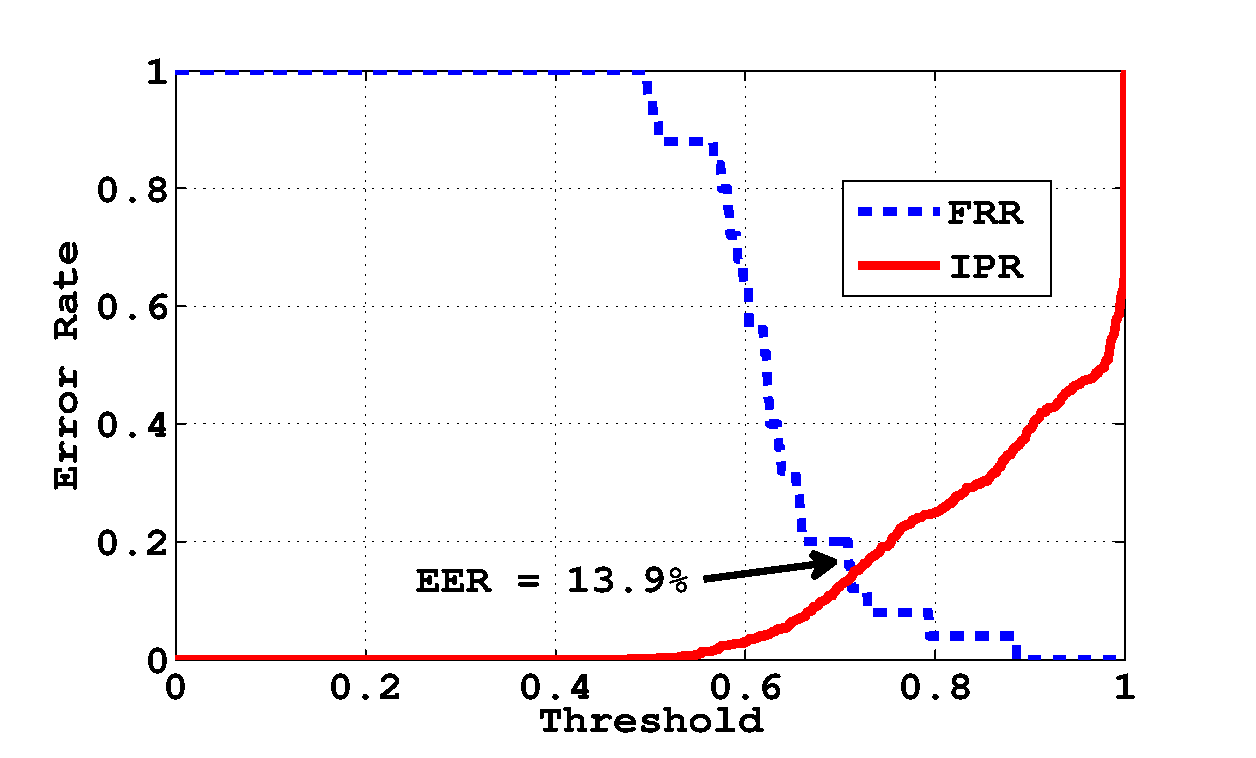
\includegraphics[width=.8\linewidth]{M1}
  \caption{Single Click $R$ = 20ms Double Click $R$ = 180ms\\M-Value = 1}
  \label{fig:sfig3}
\end{subfigure}%
\begin{subfigure}{.5\textwidth}
  \centering
  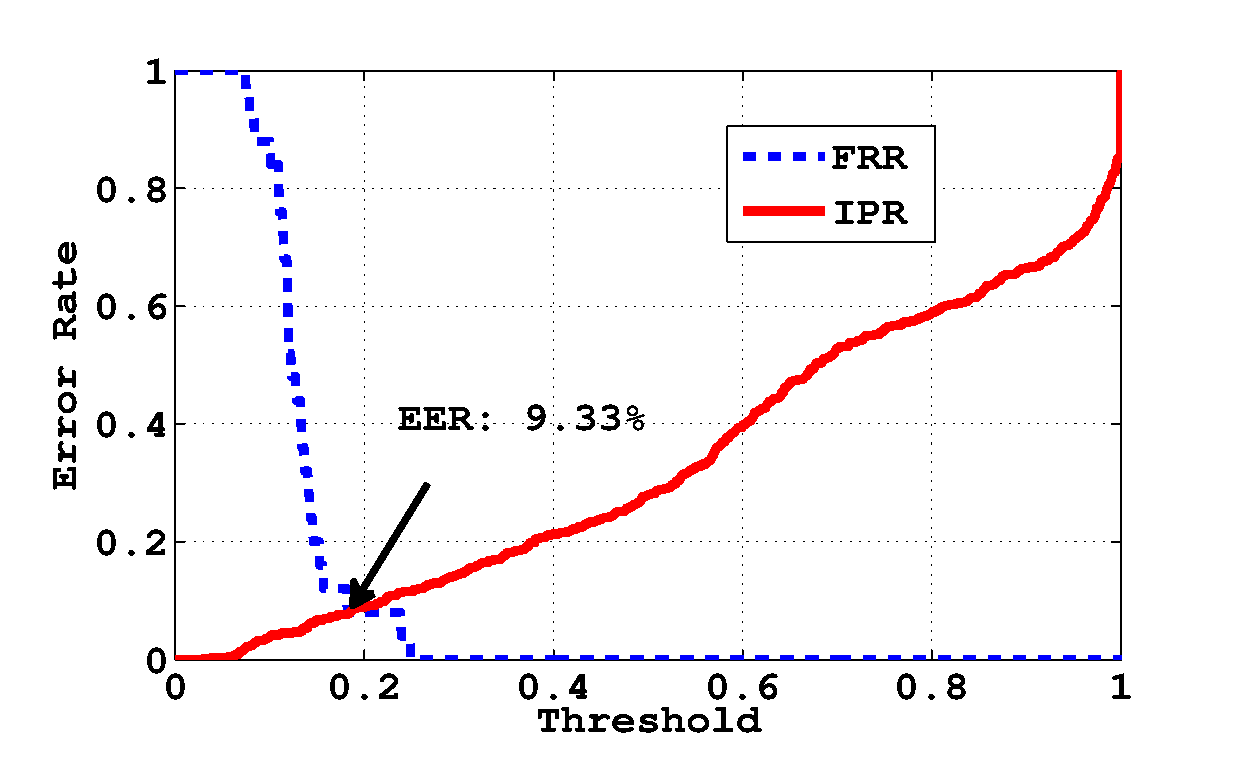
\includegraphics[width=.8\linewidth]{19M}
  \caption{Single Click $R$ = 30ms Double Click $R$ = 190m\\ M-Value = 1.9}
  \label{fig:sfig4}
\end{subfigure}
\caption{Plots of the IPR and the FRR for four different parameter settings. The point at which the IPR and FRR intersect is the Equal Error Rate (EER). }
\label{fig:fig}
\end{figure*}



\section{Methodology}


\subsection{Outlier Filtering}

For our setup we first went through each of the user samples and extracted each of the features from each mouse movement. To remove rare cases of features far from the normal, we implemented an outlier removal scheme. We define a mouse feature to be an outlier if it is more eccentric than 66\% of the population of the same mouse features for a single user. For example, if we are looking to find if a particular mouse feature $F$ is an outlier we use the algorithm described in Algorithm \ref{alg:algorithm1}. 


\begin{algorithm}

\caption{Determines if a single feature $F$ is an outlier from the rest of the population of its own kind. $featurePopulation$ is an array of same-typed features from a testing sample that $F$ is also a member of.}\label{euclid}
\begin{algorithmic}[1]
\Procedure{IsAnOutlier}{$F$}
\State $\textit{count} \gets 0$
	\For{\textbf{each} $feature \textrm{ in } featurePopulation$}
			\If{$ |F - feature| > R$}
				\State $count \gets count + 1$
			\EndIf
	\EndFor
	\If{$count \div featurePopulation_{size} \ge .33$}

		\State \Return{\texttt{True}}
	\Else
		\State \Return{\texttt{False}} 

	\EndIf
\EndProcedure
\end{algorithmic}
\label{alg:algorithm1}

\end{algorithm}

We defined a variable $R$, for each mouse feature, a number large enough to include most of the population while small enough to remove the noise from the data. We found optimal values for our $R$ values after extensive experimentation we will describe later on.\\
We created a simple algorithm for determining if a particular record of a mouse feature is an outlier outlined in Algorithm \ref{alg:algorithm1}. For a given set of mouse features from a training sample (the $featurePopulation$), we compared each feature in the $featurePopulation$ against every other feature of the same type, i.e. a Single Left Click Length feature is only compared to every other Single Left Click Length feature. Then a simple tally is kept of how many of the features in the $featurePopulation$ have a distance greater than $R$ as shown on line 4 and 5 of Algorithm \ref{alg:algorithm1}. On line 6 we simple restate that if the if the tally is greater than 33\% of the $featurePopulation$ we claim the feature F is an outlier and discard it from the training set.



\begin{figure*}
\begin{subfigure}{.5\textwidth}
  \centering
  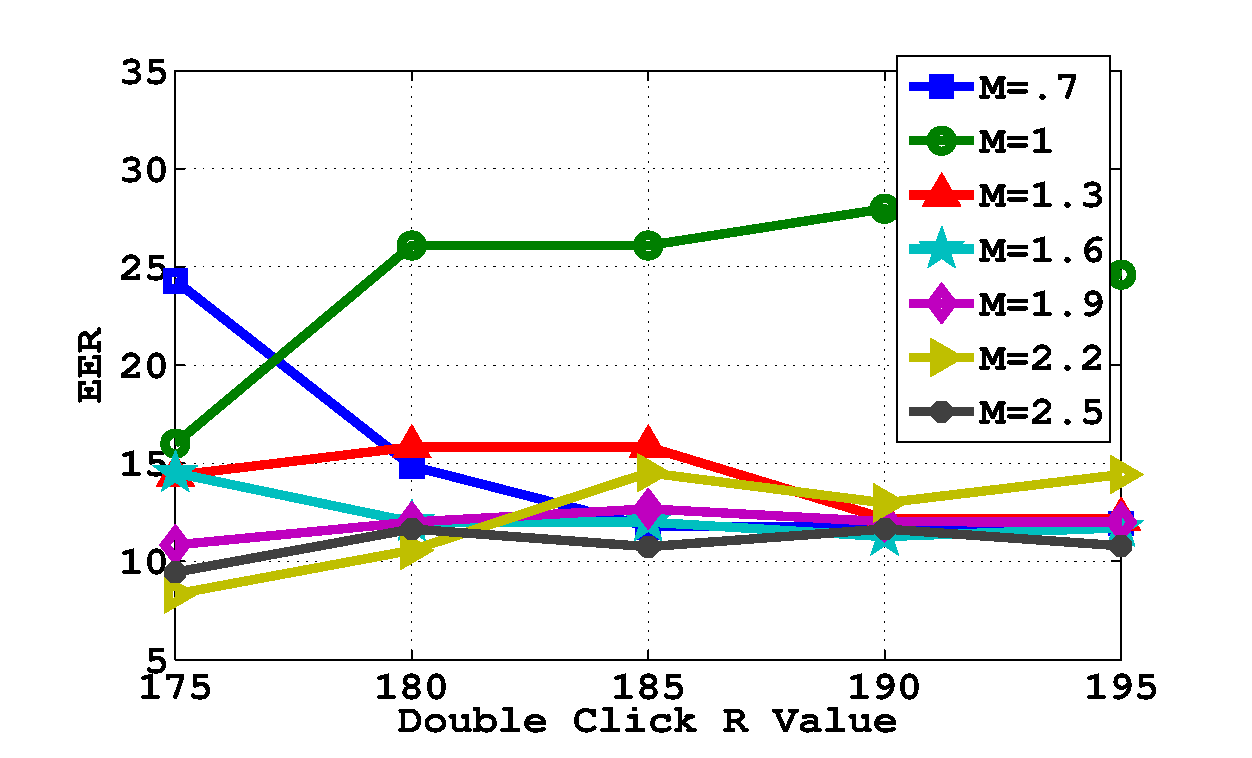
\includegraphics[width=.8\linewidth]{15.eps}
  \caption{Single Click $R$ = 15ms \\Local Max = 24.29\% Local Min = 8.33\% \\Local Average = 14.34\% Local STD = 5.08\%}
\centering
  \label{fig:sfig1}
\end{subfigure}%
\begin{subfigure}{.5\textwidth}
  \centering
  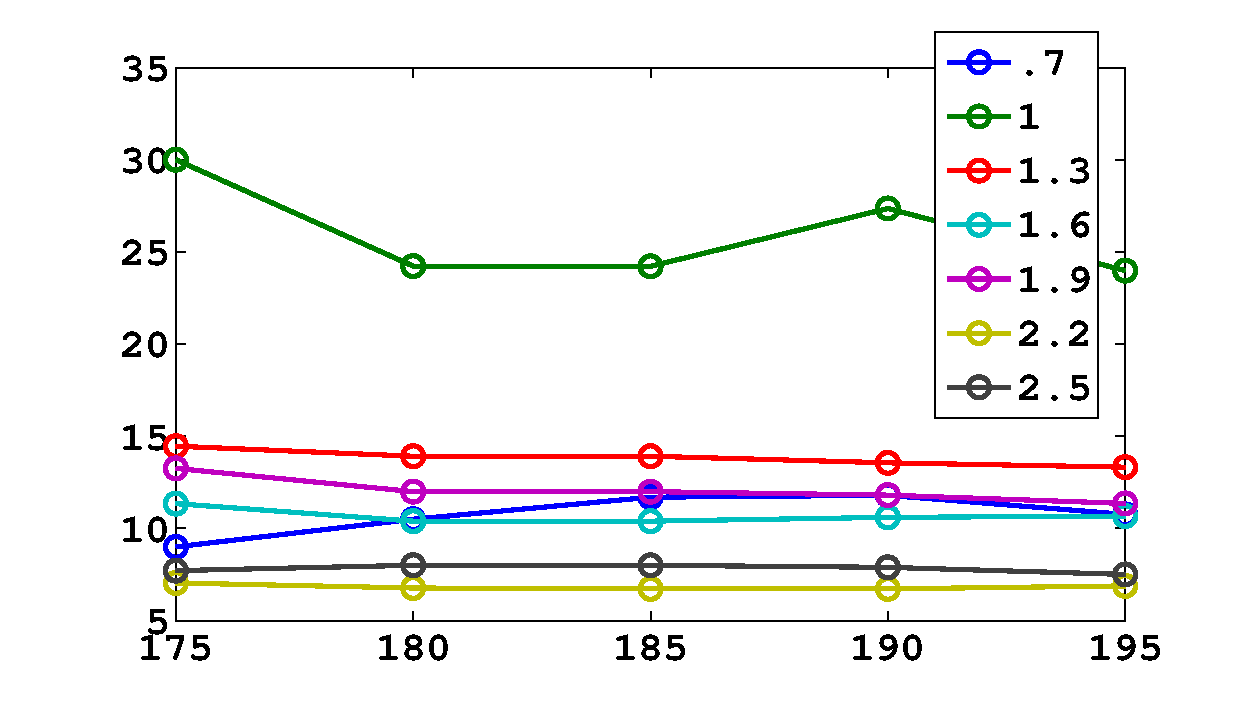
\includegraphics[width=.8\linewidth]{25.eps}
  \caption{Single Click $R$ = 25ms \\Local Max = 30.02\% Local Min = 6.77\% \\Local Average = 12.57\% Local STD = 6.07\%}
  \label{fig:sfig2}
\end{subfigure}
\begin{subfigure}{.5\textwidth}
  \centering
  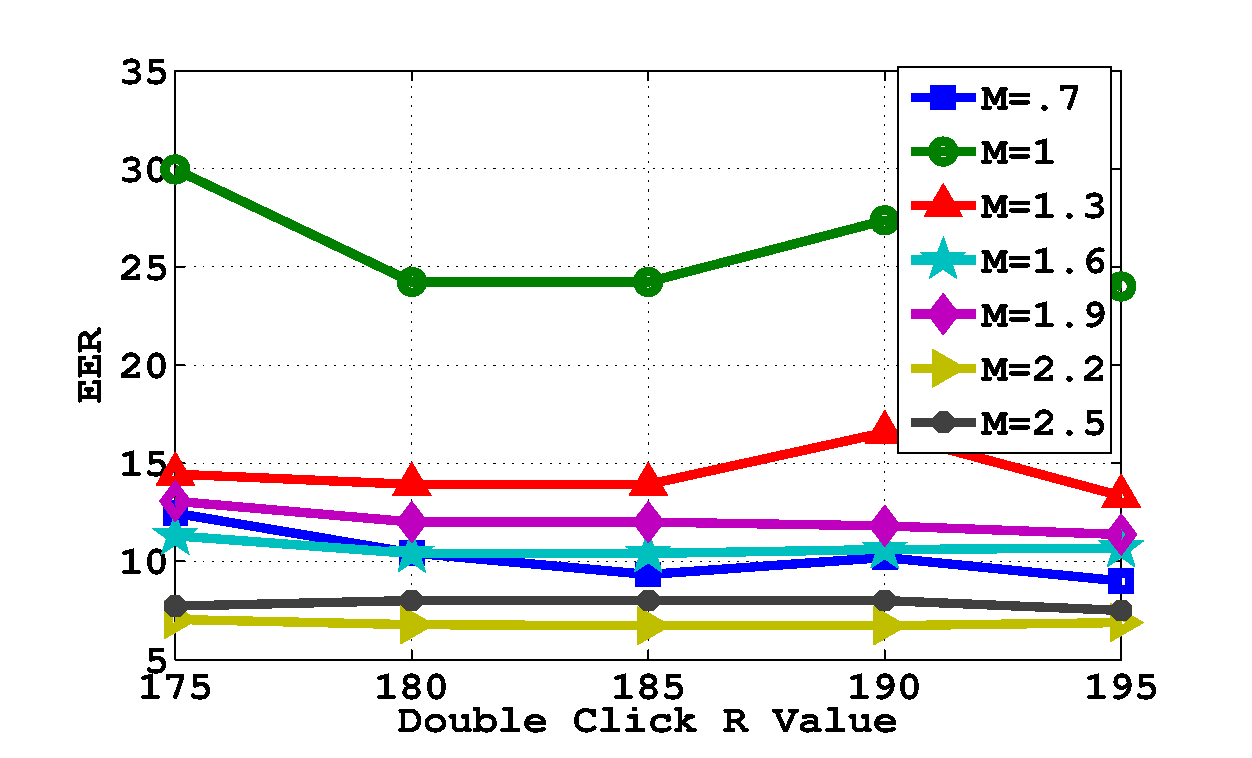
\includegraphics[width=.8\linewidth]{30.eps}
  \caption{Single Click $R$ = 30ms \\Local Max = 29.96\% Local Min = 6.70\% \\Local Average = 12.58\% Local STD = 6.13\%}
  \label{fig:sfig3}
\end{subfigure}%
\begin{subfigure}{.5\textwidth}
  \centering
  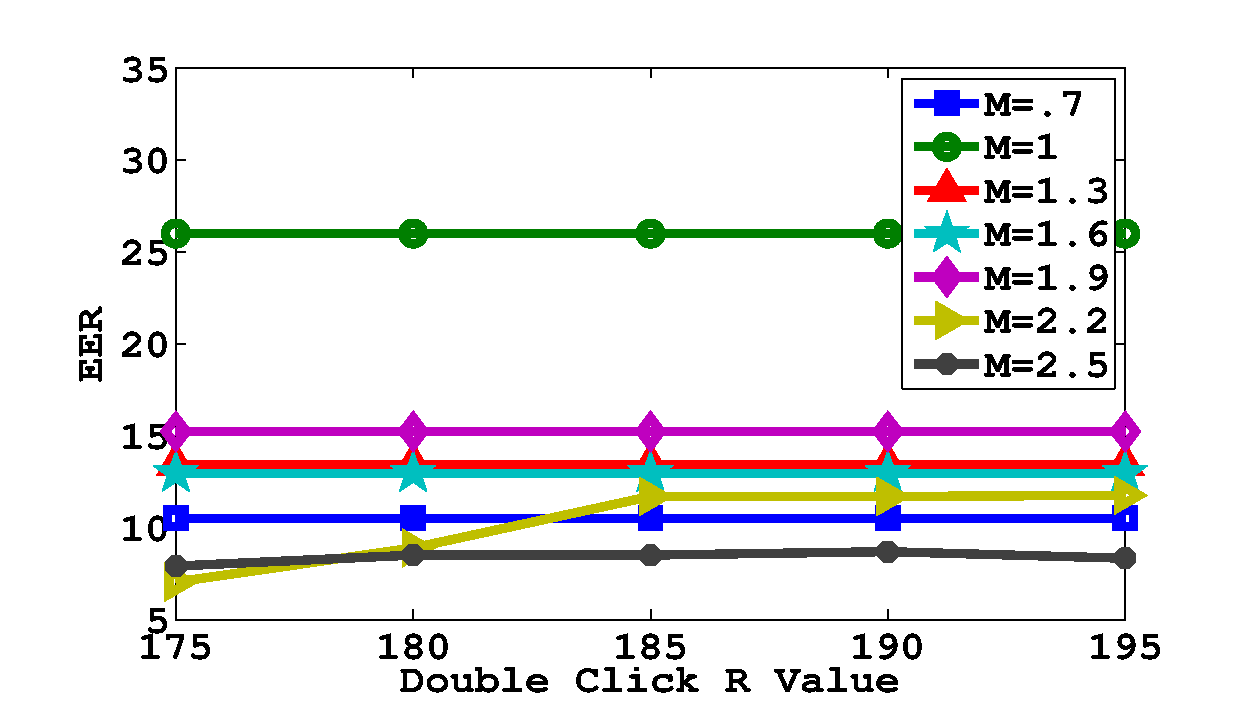
\includegraphics[width=.8\linewidth]{35.eps}
  \caption{Single Click $R$ = 35ms \\Local Max = 26\% Local Min = 7.04\%\\Local Average = 13.82\% Local STD = 5.54\%}
  \label{fig:sfig4}
\end{subfigure}
\caption{Scatter plots of EER over the ranges of the parameter values we chose. The X-axis is Double Click R-Values, the Y-axis is the EER. Each plot is a separate Single Click $R$ value. \\Global Max = 30.02\% Global Min = 6.70\% Global Average = 13.19\% Global STD = 5.77\%}
\label{fig:eer}
\end{figure*}




\subsection{Verification}
	To authenticate a user based on their mouse movements, we analyze six mouse features over the course of a sample. Our method is a simplistic user-authentication model. We create a profile based on a user's past behavior then test further samples against that profile to determine if the sample we test with is close enough to the previous profile to be considered the same user. In a real world set-up the method would look similar to Figure \ref{fig:process}. Instead, we use half of the recorded mouse movements as a test set for a user and the other half are used to train the user's profile.
We then split the edited list of features into a testing set and a training set. For each file we create user profiles based on half of the user's sample (about 50 mouse movements on average for our samples). The profiles being simply the averages and standard deviations of each of the mouse features. The mouse movements from the sample that we did not use for the profile go into the user's testing set.
Using a simple classification scoring method we can see how well a user profile and a testing set of data match up. For our entire set of data we took every user profile and tested each against every testing set. Our custom testing method generated a score for each test between 0 and 1 based on a simple scoring formula 
\begin{equation} 
score = \frac{\text{Number Of Accepted Features}}{\text{Total Number Of Features}}
\end{equation}

1 being a perfect match and 0 being a perfect mismatch. It should be noted we accept a particular feature if

\begin{equation}
\begin{split}
\begin{gathered}
   lowerBound \leq featureValue \leq upperBound, \text{where},\\
   lowerBound = AVG_{Train} - M * STD_{Train}\\
   upperBound = AVG_{Train} + M * STD_{Train}
\end{gathered}
\end{split}
\end{equation}


We tested by comparing each of the mouse movements in a testing set against the users profile. If the features in the mouse movement are within $M$ standard deviations of the corresponding means in the user profile then the test gets a point. The total amount of points accrued is divided by the total amount of mouse movements in the file to generate the score.
	




\section{Experimental Setup}
We had a few parameters where it was not immediately apparent what we should set them as. For the $R$ variables we needed values that can discriminate mouse feature values that are too eccentric while keeping as much unique data as possible. To solve this we wrote a script that ran the feature extraction and verification programs and found the EER over an array of values for each parameter to determine the optimal values for those parameters where the EER is at its lowest. We found that an $M$ value of 1.9, a Single Click $R$ of 20ms, and a Double Click $R$ of 185ms to produce the lowest EER for our set of data. By varying the parameter value we experimented with 175 (5 Single Click $R$ $\times$ 5 Double Click $R$ $\times$ 7 $M$ Values) different experimental set-ups. Note that we do not use any $R$ parameter for the other features since they show less variance. In total, we experimented with 354,357 verification attempts (45 users $\times$ 45 users $\times$ 175 experimental setups).

\begin{table}
\centering
\captionof{table}{The values used for our parameters for testing. }
\def\arraystretch{1.5}
\begin{tabular}{ l| l}
\textbf{Parameter}              &\textbf{Values Tested} \\
\hline
Single click $R$ value		& 15 20 25 30 25  \\
Double click $R$ value	& 175 180 185 190 195\\
M value		& 0.7 1 1.3 1.6 1.9 2.2 2.3\\
\end{tabular}
\end{table}




\section{Experimental Results and Analysis}

To calculate the results of our experiment we took each users profile and tested that against every other set of testing data. Therefore, for experimental setup, we generated 2025 (45 $\times$ 45) verification scores. We then calculated the False Reject Rate (FRR) and Impostor Pass Rate (IPR) values for varying threshold values from 0 to 1 with a stepsize of 0.01. We plotted 1000 FRR and IPR values as shown in each subfigure in Figure 3. For space constraint, we show FRRs and IPRs for four experimental setup out of 175 setups. In each subfigure, the EER is marked as the crossover point between FRR and IPR curves. In total, we generated 175 EERs from all setups. In Table IV, 35 EER values generated by varying double click $R$ and $M$ values when single click value set to 20ms, are listed. In Figure 4, EER values are shown for four other single click $R$ values. From the figures, our observations are as follows:

\begin{description}
  \item[$\bullet$] The Lowest EER achieved is 6.70\% (see Figure 4(c)) when $M$= 2.2, single click $R$=20ms and double click $R$=185ms. Average EER is 13.19\% and standard deviation is 5.77\%. 
  \item[$\bullet$] Among the parameters, $M$ is found to have greater influence on accuracy (see the curves in each subfigure in Figure 4). This urges to explore setting up the $M$ value for each user seperately rather than deploying generic one.
  \item[$\bullet$] Single click R value also show some level of influence on accuracy. EERs in Figure 4 (b, c) are lower than EERs in Figure 4 (a, d). It is worth mentioning that, number of single clicks are found to be far more than other activities.        

\end{description} 


\begin{table}[t]
\captionof{table}{The EER rates found across multiple parameter values. Each column is a separate double click $R$ value while each row is a separate $M$ value. The entire table is tested against one single click $R$ value set to 20ms.}
\def\arraystretch{1.5}
\addvbuffer[12pt 8pt]{\begin{tabular}{ c  l | l l l l l }


         \multirow{11}{*}{\begin{sideways} \textbf{ $M$ values}\end{sideways}} & \multicolumn{6}{c}{\textbf{Double click $R$ values}} \\


       && \textbf{175}  &  \textbf{180}  &  \textbf{185}  &  \textbf{190}  &  \textbf{195} \\
\cline{2-7}
 
   & \textbf{.7}	&14.86\%	&10.53\%	&9.33\%	&9.33\%	&8.99\%\\
   &\textbf{1}	&30.02\%	&24.23\%	&24.23\%	&27.37\%	&24.00\%\\
  &\textbf{1.3}	&14.46\%	&13.90\%	&10.40\%	&13.56\%	&13.33\%\\
   &\textbf{1.6}	&11.35\%	&10.40\%	&10.40\%	&10.59\%	&11.81\%\\
   &\textbf{1.9}	&13.35\%	&12.00\%	&12.00\%	&11.81\%	&11.36\%\\
   &\textbf{2.2}	&13.36\%	&6.77\%	&6.70\%	&\%	&6.88\%\\
  & \textbf{2.5}	&7.71\%	&8.00\%	&8.00\%	&7.89\%	&7.50\%\\
\end{tabular}}
\end{table}




\section{Conclusion}

Our comprehensive experiment which comprises 354,357 verification attempts carried over 45 users, shows the effectiveness of our method. On average, the EER we found was 13.42\%. The lowest EER was found to be 6.70\%. In future, we want to test our method on more user samples. To improve accuracy even further, we want to set the parameter values (especially $M$) for each users separately instead of adopting generic values. We believe that, a simple system with impressive accuracy such as ours, can easily be considered for continuously verify system users in real time.    

\begin{thebibliography}{100} % 100 is a random guess of the total number of
%references
\bibliographystyle{ieeetr}

\bibitem{CS} Chao Shen, Zhongmin Cai, Xiaohong Guan, Youtian Du and R. Maxion, 'User Authentication Through Mouse Dynamics', IEEE Trans.Inform.Forensic Secur., vol. 8, no. 1, pp. 16-30, 2013.
\bibitem{Jor} Z. Jorgensen and T. Yu, 'On mouse dynamics as a behavioral biometric for authentication', Proceedings of the 6th ACM Symposium on Information, Computer and Communications Security - ASIACCS '11, pp. 476-482, 2011.
\bibitem{Sch}D. Schulz, 'Mouse Curve Biometrics', 2006 Biometrics Symposium: Special Session on Research at the Biometric Consortium Conference, 2006.
\bibitem{Pus}M. Pusara and C. Brodley, 'User re-authentication via mouse movements', Proceedings of the 2004 ACM workshop on Visualization and data mining for computer security - VizSEC/DMSEC '04, 2004.
\bibitem{She}C. Shen, Z. Cai, X. Guan, H. Sha and J. Du, 'Feature Analysis of Mouse Dynamics in Identity Authentication and Monitoring', 2009 IEEE International Conference on Communications, 2009.
\bibitem{Ahmed} A. Ahmed and I. Traore, 'A New Biometric Technology Based on Mouse Dynamics', IEEE Trans. Dependable and Secure Comput., vol. 4, no. 3, pp. 165-179, 2007.
\bibitem{Zhe}N. Zheng, A. Paloski and H. Wang, 'An efficient user verification system via mouse movements', Proceedings of the 18th ACM conference on Computer and communications security - CCS '11, pp. 139-150, 2011.
\bibitem{Nak}Y. Nakkabi, I. Traore and A. Ahmed, 'Improving Mouse Dynamics Biometric Performance Using Variance Reduction via Extractors With Separate Features', IEEE Trans. Syst., Man, Cybern. A, vol. 40, no. 6, pp. 1345-1353, 2010.
\bibitem{Syu}A. Syukri, E. Okamoto and M. Mambo, 'A user identification system using signature written with mouse', Information Security and Privacy, pp. 403-414, 1998.
\bibitem{HJ} H. Jahankhani, D. Palmer-Brown and K. Revett, 'A Survey of User Authentication Based on Mouse Dynamics', Global E-Security. Berlin, Heidelberg: Springer-Verlag Berlin Heidelberg, 2008, pp. 210-219.



\end{thebibliography}


\end{document}